\chapter{复数}

本章介绍复数。难点和平面向量一样,所以依然是反复研读定义,多画图。其次要注意和向量的区别。

本章要点:
\begin{itemize}
    \item 复数及其几何意义。
\end{itemize}

\newpage
\section{复数的概念}

本节要点:
\begin{itemize}
    \item 掌握复数的概念;
    \item 熟悉复数的几何意义;
    \item 理解复数和向量的关系。
\end{itemize}

~

\[
z=a+bi
\]

复数的定义没啥难点,数学家已经帮我们起头了。复数的发明XML。

复数的几何意义对应一个二维平面,但特别注意,由于复数的乘法和向量的乘法(内积)定义不同,所以复数和向量不是同构的,因此,我们称复数的几何表示为复平面,称向量的几何表示为二维平面!XML。

学习到这里一定要注意区别复数和向量。

\begin{tcolorbox}
复数的物理意义需要在解微分方程时讨论,超出高中数学的范围,所以高中阶段不讨论复数的物理意义。我们需要知道,复数确实有物理意义,很多物理现象都涉及复数,XML。
\end{tcolorbox}

~

\begin{example}[拓广探索11,难度:$\star $]
在复平面内指出与复数$z_1=1+2i,z_2=\sqrt{2}+\sqrt{3}i,z_3=\sqrt{3}-\sqrt{2}i,z_4=-2+i$对应的点$z_1,z_2,z_3,z_4$,判断这4个点是否在同一个圆上,并证明你的结论。
\end{example}

解:

在同一个圆上,且圆心为原点。
\[
\left| z_1 \right|=\left| z_2 \right|=\left| z_3 \right|=\left| z_4 \right|=\sqrt{5}
\]

\begin{tcolorbox}
此题非常放水,圆心在原点,直接判断模,非常简单。
\end{tcolorbox}






\newpage
\section{复数的四则运算}

本节要点:
\begin{itemize}
    \item 掌握复数的运算法则;
    \item 理解复数运算的几何意义。
\end{itemize}

~

复数的加减和向量加减一样,但乘除和向量完全不同。
\begin{align*}
&z_1\pm z_2=\left( a_1\pm a_2 \right) +\left( b_1\pm b_2 \right) i \\
&z_1\cdot z_2=\left( a_1+b_1i \right) \cdot \left( a_2+b_2i \right) =\left( a_1a_2-b_1b_2 \right) +\left( a_1b_2+a_2b_1 \right) i
\end{align*}

加法的交换律和结合律:
\begin{align*}
&z_1+z_2=z_2+z_1 \\
&\left( z_1+z_2 \right) +z_3=z_1+\left( z_2+z_3 \right)
\end{align*}

数乘的结合律和分配律:
\begin{align*}
&\lambda \left( \mu z \right) =\left( \lambda \mu \right) z \\
&\left( \lambda +\mu \right) z=\lambda z+\mu z \\
&\lambda \left( z_1+z_2 \right) =\lambda z_1+\lambda z_2
\end{align*}

乘法的交换律、结合律和分配律:
\begin{align*}
&z_1z_2=z_2z_1 \\
&\left( z_1z_2 \right) z_3=z_1\left( z_2z_3 \right) \\
&z_1\left( z_2+z_3 \right) =z_1z_2+z_1z_3
\end{align*}

一个重要的不等式和一个重要的等式:
\begin{itemize}
    \item $\left| z_1+z_2 \right|\leqslant \left| z_1 \right|+\left| z_2 \right|$,当且仅当$z_1,z_2$重叠时等号成立;
    \item $\left| z_1\cdot z_2 \right|=\left| z_1 \right|\cdot \left| z_2 \right|$。
\end{itemize}
注意和向量的区别。






\newpage
\section{复数的三角表示}

本节要点:
\begin{itemize}
    \item 用三角表示理解复数的乘除。
\end{itemize}

~

三角表示及乘除运算如下:
\begin{align*}
&z=a+bi=r\left( \cos \theta +i\sin \theta \right) \\
&z_1\cdot z_2=r_1r_2\left[ \cos \left( \theta _1+\theta _2 \right) +i\sin \left( \theta _1+\theta _2 \right) \right] \\
&\frac{z_1}{z_2}=\frac{r_1}{r_2}\left[ \cos \left( \theta _1-\theta _2 \right) +i\sin \left( \theta _1-\theta _2 \right) \right]
\end{align*}
显然,复数的乘除的几何意义在于旋转。

~

\begin{example}[拓广探索9,难度:$\star $]
如下图,复平面内的$\bigtriangleup ABC$是等边三角形,它的两个顶点$A,B$的坐标分别为$\left( 1,0 \right) ,\left( 2,1 \right) $,求点$C$的坐标。
\end{example}

\begin{figure}[h]
\centering
\begin{minipage}{.49\textwidth}
\centering
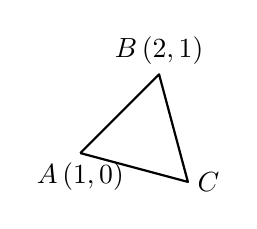
\begin{tikzpicture}[line join=round, scale=1]
\mydrawxy{-0.5}{3}{-0.5}{1.3}
\coordinate[label=below:{$A\left( 1,0 \right) $}] (A) at (1,0);
\coordinate[label=above:{$B\left( 2,1 \right) $}] (B) at (2,1);
\coordinate[label=right:{$C$}]                    (C) at (2.366,-0.366);
\draw[thick] (A)--(B)--(C)--(A);
\end{tikzpicture}
\end{minipage}
\begin{minipage}{.49\textwidth}
\centering
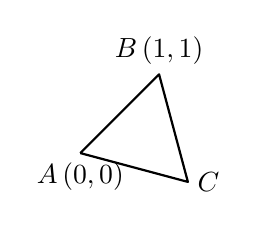
\begin{tikzpicture}[line join=round, scale=1]
\mydrawxy{-0.5}{2}{-0.5}{1.3}
\coordinate[label=below:{$A\left( 0,0 \right) $}] (A) at (0,0);
\coordinate[label=above:{$B\left( 1,1 \right) $}] (B) at (1,1);
\coordinate[label=right:{$C$}]                    (C) at (1.366,-0.366);
\draw[thick] (A)--(B)--(C)--(A);
\end{tikzpicture}
\end{minipage}
\end{figure}

解:

不妨平移坐标,如上右图,不难得到:
\begin{align*}
&z_B=\sqrt{2}\left( \cos \frac{\pi}{4}+i\sin \frac{\pi}{4} \right) \\
&z_C=\sqrt{2}\left[ \cos \left( -\frac{\pi}{12} \right) +i\sin \left( -\frac{\pi}{12} \right) \right]
\end{align*}
$C$在第四象限,于是:
\begin{align*}
&\cos \left( -\frac{\pi}{12} \right) =\sqrt{\frac{1+\cos \frac{\pi}{6}}{2}}=\sqrt{\frac{1}{2}+\frac{\sqrt{3}}{4}} \\
&\sin \left( -\frac{\pi}{12} \right) =-\sqrt{\frac{1-\cos \frac{\pi}{6}}{2}}=-\sqrt{\frac{1}{2}-\frac{\sqrt{3}}{4}} \\
&z_C=\sqrt{1+\frac{\sqrt{3}}{2}}-\sqrt{1-\frac{\sqrt{3}}{2}}i
\end{align*}
将坐标轴反向移回,得到$C$的最终坐标:
\[
z_C=\sqrt{1+\frac{\sqrt{3}}{2}}+1-\sqrt{1-\frac{\sqrt{3}}{2}}i
\]

\begin{tcolorbox}
本题也可以用向量求解,关键在于平移坐标系降低运算量。
\end{tcolorbox}

~

\begin{example}[拓广探索10,难度:$\star $]
如下图,已知平面内并列的三个全等的正方形,利用复数证明
\[
\angle 1+\angle 2+\angle 3=\frac{\pi}{2}
\]
\end{example}

\begin{figure}[h]
\centering
\begin{tikzpicture}[line join=round, scale=1.25]
\mydrawxy{-0.5}{3.5}{-0.5}{1.3}
\coordinate[label=below left:{$O$}] (A0) at (0,0);
\coordinate[label=below:     {$1$}] (A1) at (1,0);
\coordinate[label=below:     {$2$}] (A2) at (2,0);
\coordinate[label=below:     {$3$}] (A3) at (3,0);
\coordinate[label=left:      {$1$}] (B0) at (0,1);
\coordinate                         (B1) at (1,1);
\coordinate                         (B2) at (2,1);
\coordinate                         (B3) at (3,1);
\draw[thick] (A0)--(A3)--(B3)--(B0)--(A0) (A1)--(B1) (A2)--(B2) (A3)--(B3);
\draw[dashed] (A0)--(B1) (A0)--(B2) (A0)--(B3);
\pic["$1$",draw,angle radius=0.5cm,angle eccentricity=1.5] {angle=B0--B1--A0};
\pic["$2$",draw,angle radius=0.5cm,angle eccentricity=1.5] {angle=B0--B2--A0};
\pic["$3$",draw,angle radius=0.5cm,angle eccentricity=1.5] {angle=B0--B3--A0};
\end{tikzpicture}
\end{figure}

解:

令$z_1=1+i,z_2=2+i,z_3=3+i$,使用复数乘法的几何意义:
\[
z_1z_2z_3=\left( 1+i \right) \left( 2+i \right) \left( 3+i \right) =10i
\]
证毕。

\begin{tcolorbox}
本题考察复数乘法的几何意义,非常简单。
\end{tcolorbox}






\newpage
\section{本章小结}

本章介绍了复数,重点在于复数的运算及其几何意义。复数也是一个全新的域,同样需要反复阅读概念并结合几何深入思考,同时需要和向量在乘除上的区别。

我们将向量和复数的运算的几何意义归纳如下。

\begin{table}[ht]
\centering
\begin{tabular}{ccc}
    \toprule
     & 向量 & 复数\\
    \midrule
    加减 & 平行四边形对角线 & 平行四边形对角线\\
    乘法 & 判断直角 & 旋转\\
    除法 & 无 & 旋转\\
    \bottomrule
\end{tabular}
\end{table}

根据具体形况,使用向量判断线段关系,还是使用复数计算线段夹角,需要具体问题具体分析。

~

\begin{example}[拓广探索9,难度:$\star \star \star $]
已知复数
\begin{align*}
&z_1=m+\left( 4-m^2 \right) i \qquad m\in \mathbb{R} \\
&z_2=2\cos \theta +\left( \lambda +3\sin \theta \right) i \qquad \lambda ,\theta \in \mathbb{R}
\end{align*}
并且$z_1=z_2$,求$\lambda $的取值范围。
\end{example}

解:

先考察两个复数的几何图形,均是参数方程,转化为普通方程:
\begin{align*}
&z_1:\begin{cases}
	x=m\\
	y=4-m^2\\
\end{cases}\Rightarrow \quad y=4-x^2 \\
&z_2:\begin{cases}
	x=2\cos \theta\\
	y=\lambda +3\sin \theta\\
\end{cases}\Rightarrow \quad \left( \frac{x}{2} \right) ^2+\left( \frac{y-\lambda}{3} \right) ^2=1
\end{align*}
一个开口向下的抛物线,一个椭圆。$\lambda $控制了椭圆的沿{\it y}轴的平移,要使$z_1=z_2$,即两个图形要相交,$x,y$均需有实数解。几何意义虽然明显,但全靠几何求解很难,考察代数方法,上式带入下式得到:
\[
\frac{4-y}{4}+\left( \frac{y-\lambda}{3} \right) ^2=1
\]
$y$必须在$y\leqslant 4$有实数解
\begin{align*}
&\frac{4-y}{4}+\left( \frac{y-\lambda}{3} \right) ^2=1 \\
&4y^2-\left( 8\lambda +9 \right) y+4\lambda ^2=0 \\
&\because \Delta =\left( 8\lambda +9 \right) ^2-64\lambda ^2\geqslant 0 \\
&\therefore \lambda \geqslant -\frac{9}{16}
\end{align*}
另一个可由几何获得:
\[
\lambda _{\max}=4+3=7
\]
综合得到$\lambda \in \left[ -\frac{9}{16},7 \right] $。

\begin{figure}[h]
\centering
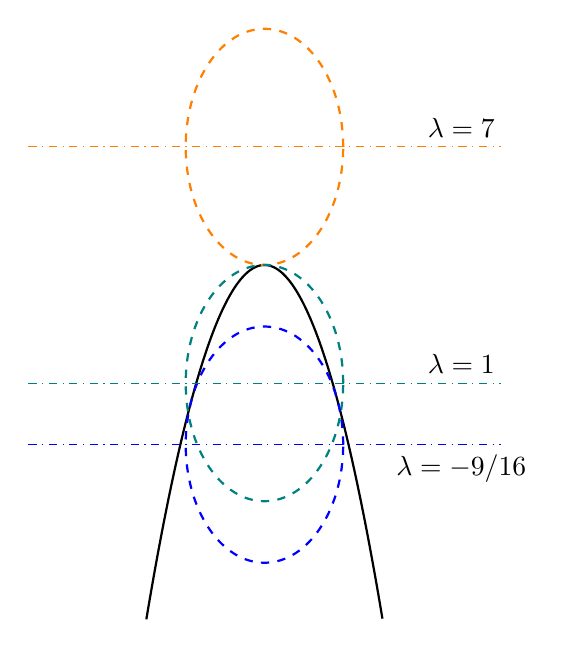
\begin{tikzpicture}[line join=round, scale=0.5]
\mydrawxy{-7}{7}{-5}{11}
\draw[thick,domain=-3:3,samples=200] plot ( \x,{4-((\x)^2)});
\draw[thick,dashed,orange] (0,7)       ellipse (2 and 3);
\draw[thick,dashed,teal]   (0,1)       ellipse (2 and 3);
\draw[thick,dashed,blue]   (0,-0.5625) ellipse (2 and 3);
\draw[dashdotted,orange] (-6,7)--(6,7);
\draw[dashdotted,teal] (-6,1)--(6,1);
\draw[dashdotted,blue] (-6,-0.5625)--(6,-0.5625);
\coordinate[label=above:{$\lambda =7$}]     (t1) at (5,7);
\coordinate[label=above:{$\lambda =1$}]     (t2) at (5,1);
\coordinate[label=below:{$\lambda =-9/16$}] (t3) at (5,-0.5625);
\end{tikzpicture}
\end{figure}

这里附带讨论交点的{\it y}坐标,如下:
\[
y=\frac{\left( 8\lambda +9 \right) \pm 3\sqrt{16\lambda +9}}{8}
\]
\begin{itemize}
    \item $\lambda <-9/16$:$y$没有实数解,两条曲线没有交点;
    \item $\lambda =-9/16$:$y_{1,2}=9/16$,两条曲线有左右2个对称的交点;
    \item $\lambda \in \left( -\frac{9}{16},1 \right) $:$y_{1,2}>0$,两条曲线有左右4个对称的交点;
    \item $\lambda =1$:$y_{1,2}=4,1/4$,两条曲线有左右2个对称的交点,和一个$\left( 0,4 \right) $,共3个交点;
    \item $\lambda \in \left( 1,7 \right) $:$y$有正有负,受$x$实数限制,取$y>0$,所以两条曲线有左右2个对称的交点;
    \item $\lambda =7$:$y_{1,2}=\frac{98}{8},4$,受$x$实数限制,取$y=4$,两条曲线只有顶部1个交点。
\end{itemize}


\begin{tcolorbox}
本题其实考察曲线的交点,结合了复数、参数方程、抛物线、椭圆。纯粹用代数非常复杂,结合几何意义就非常清晰简单。本题很有典型性,仔细研读讨论部分,XML。
\end{tcolorbox}









